%%!TEX encoding = UTF-8 Unicode 
\documentclass{beamer}
\let\Tiny=\tiny

%\mode<presentation>{
  %\usetheme{Singapore}
  %\usecolortheme{rose}
  %\usefonttheme{structurebold}
  %\setbeamertemplate{caption}[numbered]
%} 
\mode<presentation>{
  \usetheme{Boadilla}
  \usecolortheme{whale}
  \usefonttheme{structurebold}
  \setbeamertemplate{caption}[numbered]
} 

%\usepackage{pgfplots}
\usepackage{verbatim}
%\pgfplotsset{compat=1.8}
%\pgfplotsset{grid style={dashed}}

\usepackage{listings}
\lstset{
    tabsize=4,
    basicstyle=\ttfamily,
    frame=single,
    captionpos=b,
    breaklines=true,
    columns=flexible,
}

\usepackage[english]{babel}
\usepackage[utf8x]{inputenc}

\usepackage{todonotes}
\usepackage{multirow}
\usepackage{pgfpages}
\pgfpagesuselayout{resize to}[physical paper width=8in, physical paper height=6in]

\title{
    GMetis - Xeon Phi
}

\author{
    David Pereira
    \and
    Rui Brito
}

\date{\today}


\begin{document}

\begin{frame}
  \titlepage
\end{frame}

\begin{frame}{Outline}
  \tableofcontents
\end{frame}


%-----------------------------------------------------------------------------
% Introduction
%-----------------------------------------------------------------------------

\section{Introduction}

\begin{frame}{Introduction}
\begin{itemize}
    \item GMetis is a graph partitioning application which uses the Galois
      framework
    \item Consists of three major phases
      \begin{itemize}
        \item Coarsening
        \begin{itemize}
          \item Find matching nodes
          \item Create Coarse Edges
        \end{itemize}
        \item Initial Partitioning (Clustering)
        \item Refinement
      \end{itemize}
\end{itemize}
\end{frame}


%-----------------------------------------------------------------------------
% Algorithm Description
%-----------------------------------------------------------------------------

\section{Algorithm Description}

\begin{frame}{Algorithm Description}
  \begin{center}
  \begin{figure}[htbp]
      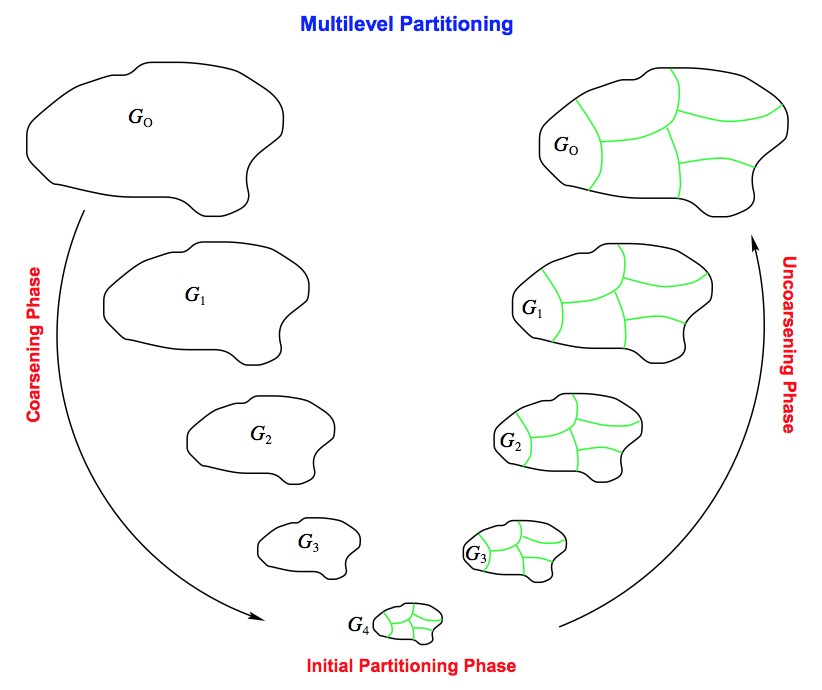
\includegraphics[scale=.5]{img/metis.png}
  \end{figure}
  \end{center}
\end{frame}

\begin{frame}{Formal Description}

\begin{itemize}
  \item Given a graph $G_0 = (V_0,E_0)$:
  \begin{itemize}    
    \item Coarsening
    \begin{itemize}
      \item $G_0$ is transformed into a sequence of smaller graphs $G_1,G_2,\cdots,G_m$ such that $|V_0|>|V_1|>|V_2|>\cdots>|V_m|$
    \end{itemize}
    \item Partitioning 
    \begin{itemize}
      \item A 2-way partition $P_m$ of the graph $G_m = (V_m,E_m)$ is computed that partitions $V_m$ into two parts, each containing half the vertices of $G_0$
    \end{itemize}
    \item Refinement
    \begin{itemize}
      \item The partition $P_m$ of $G_m$ is projected back to $G_0$ by going through intermediate partitions $P_{m-1}, P_{m-2},\cdots,P_1,P_0 $
    \end{itemize}
  \end{itemize}
\end{itemize}

\end{frame}

\begin{frame}{Coarsening}

  \begin{columns}[c]
    \column{.45\textwidth}{}
    \scriptsize
    \begin{center}
      \begin{figure}[htbp]
        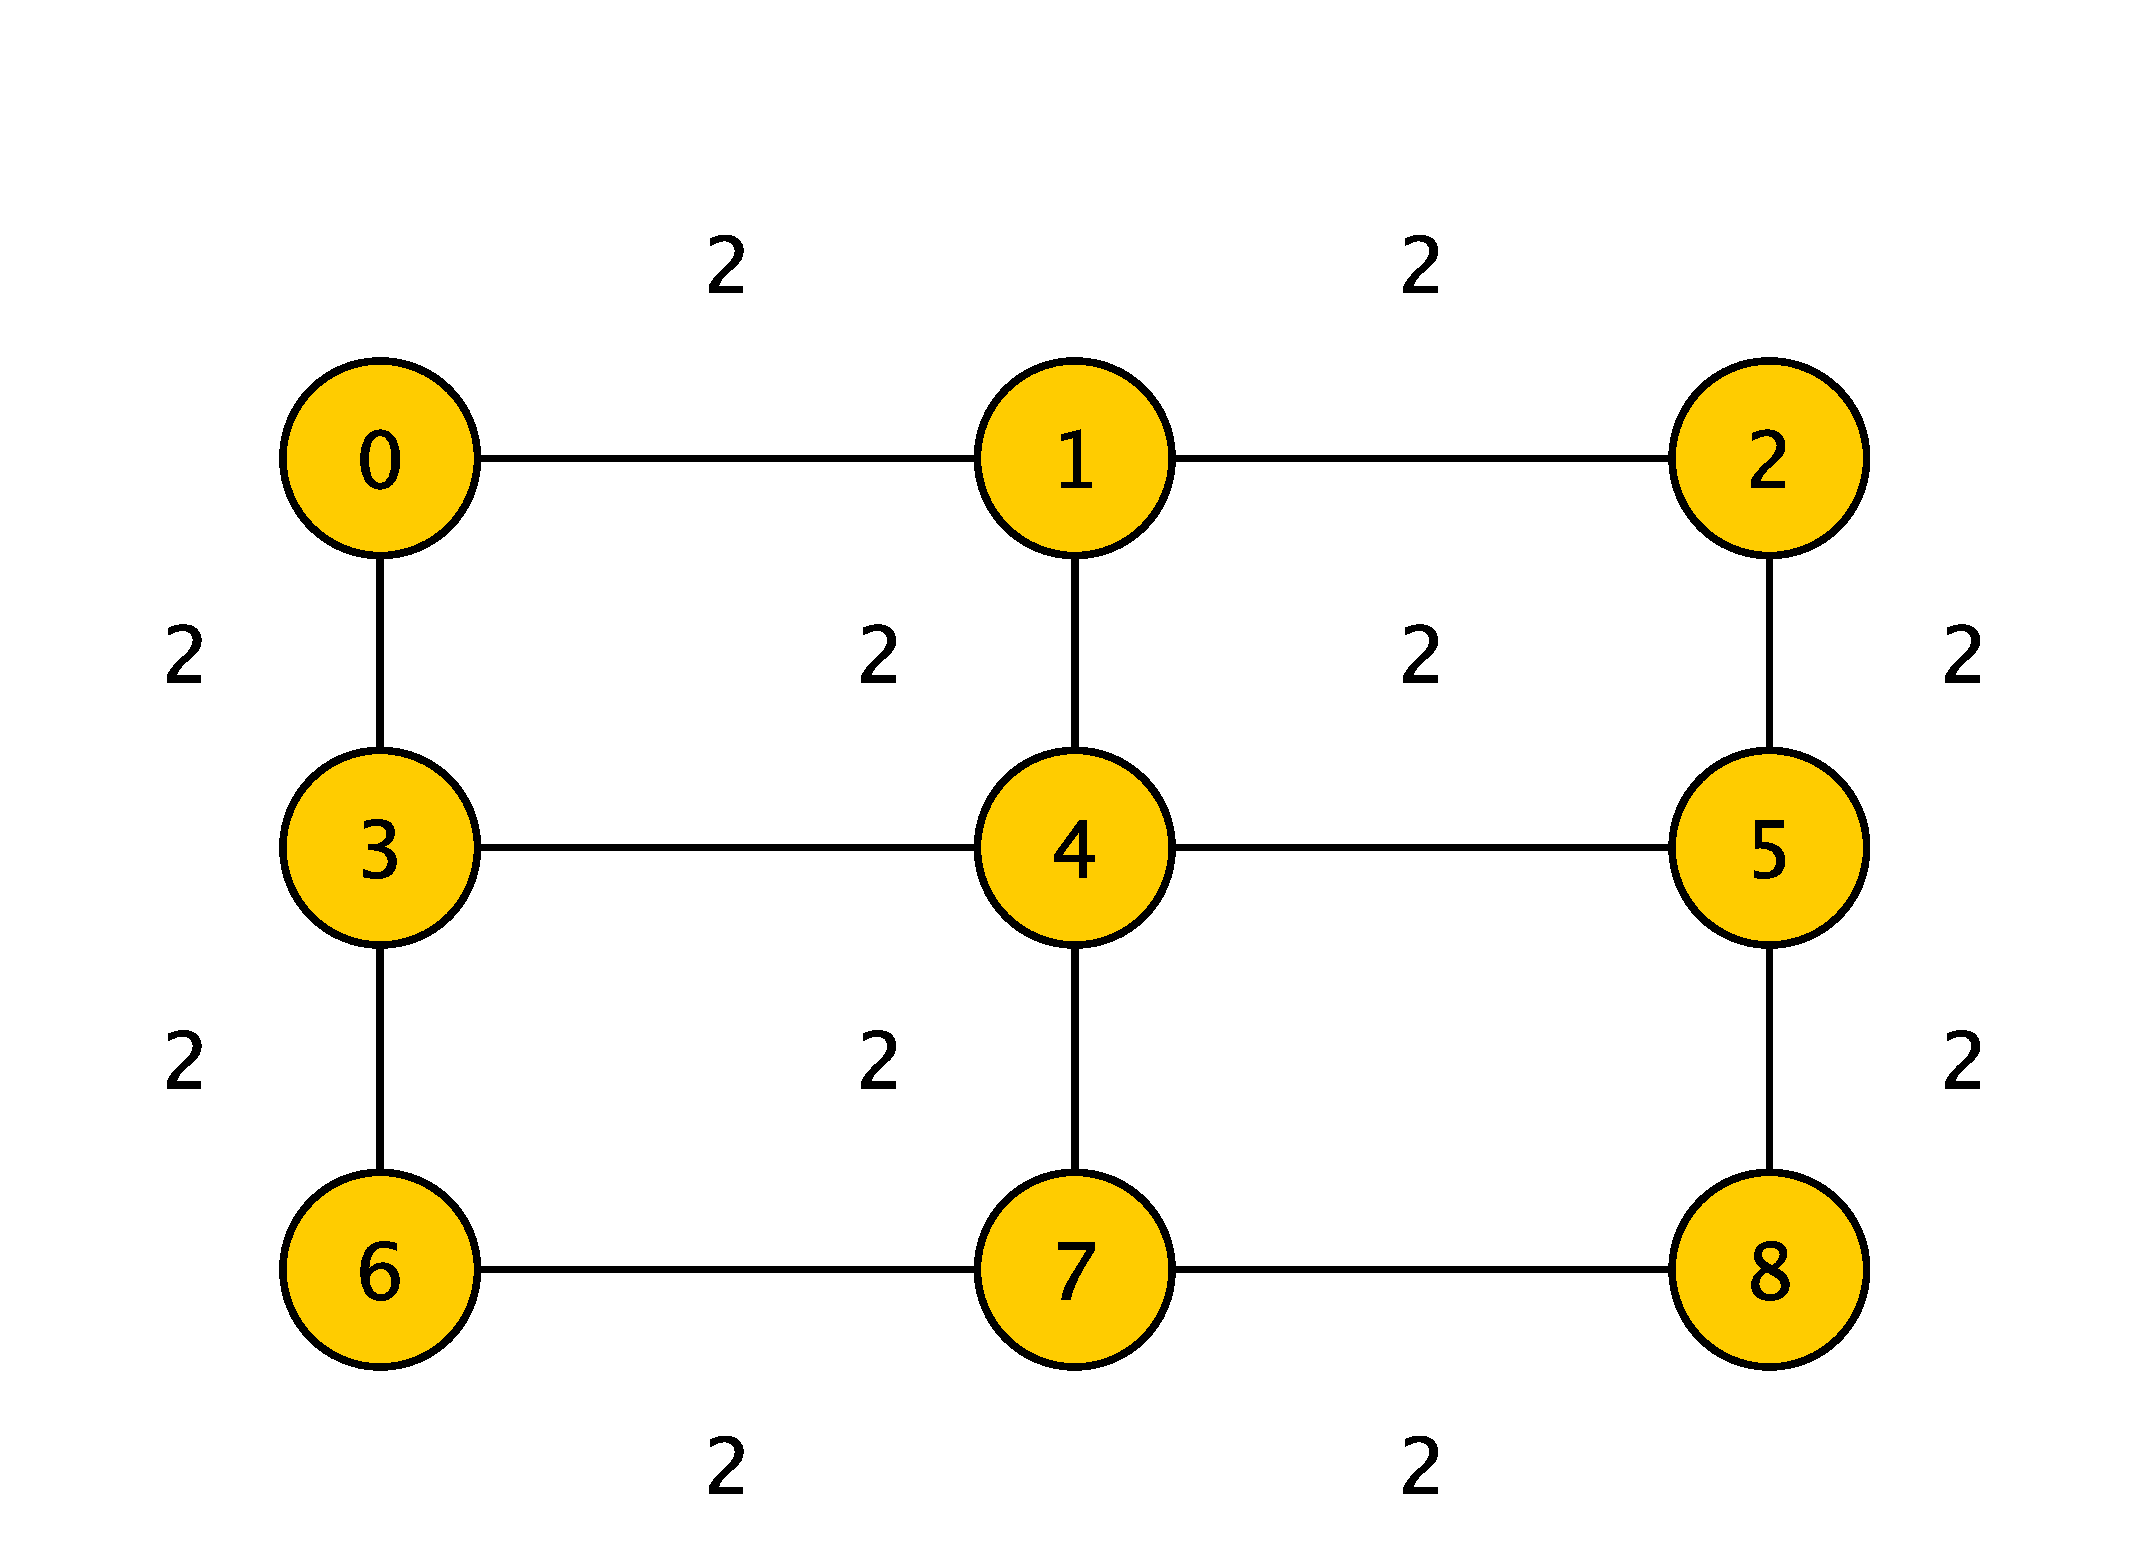
\includegraphics[scale=.15]{img/coarsening.eps}
      \end{figure}
    \end{center}

    \column{.05\textwidth}{} 
    \begin{center}
      $\longrightarrow$  
    \end{center}    
    
    \column{.45\textwidth}{} 
    \begin{center}
      \begin{figure}[htbp]
        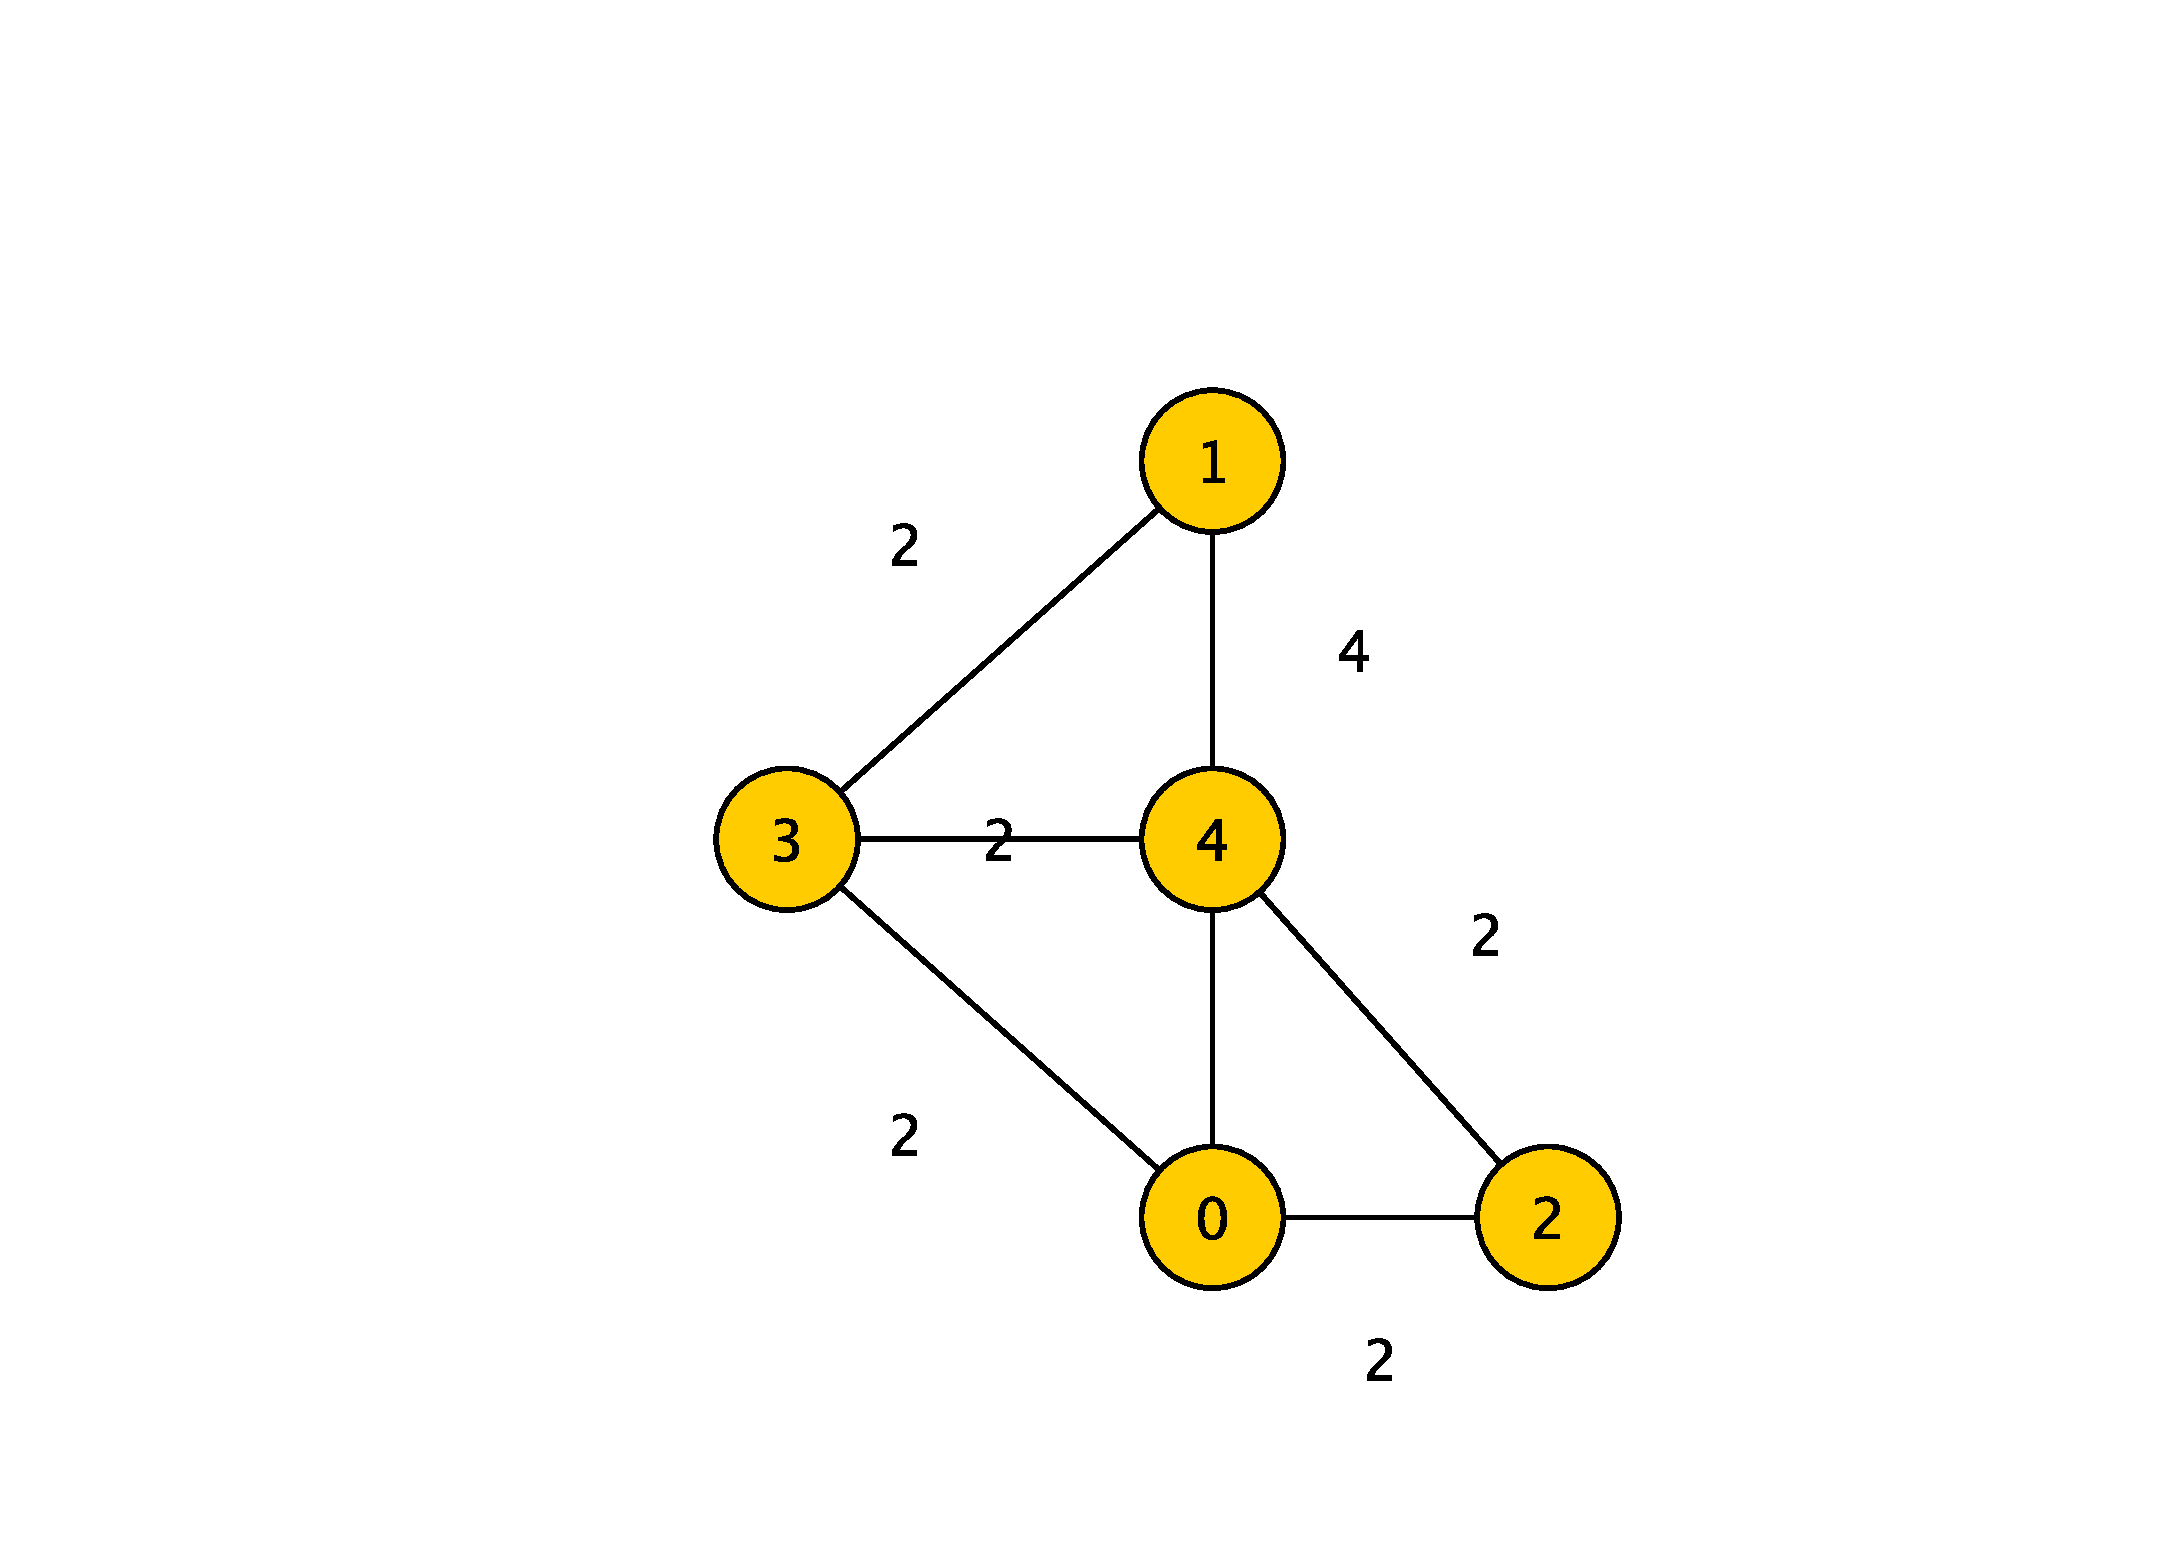
\includegraphics[scale=.15]{img/coarsening2.eps}
      \end{figure}
    \end{center}

  \end{columns}
\end{frame}



\begin{frame}{Partitioning}
  \begin{columns}[c]
    \column{.45\textwidth}{}
    \scriptsize
    \begin{center}
      \begin{figure}[htbp]
        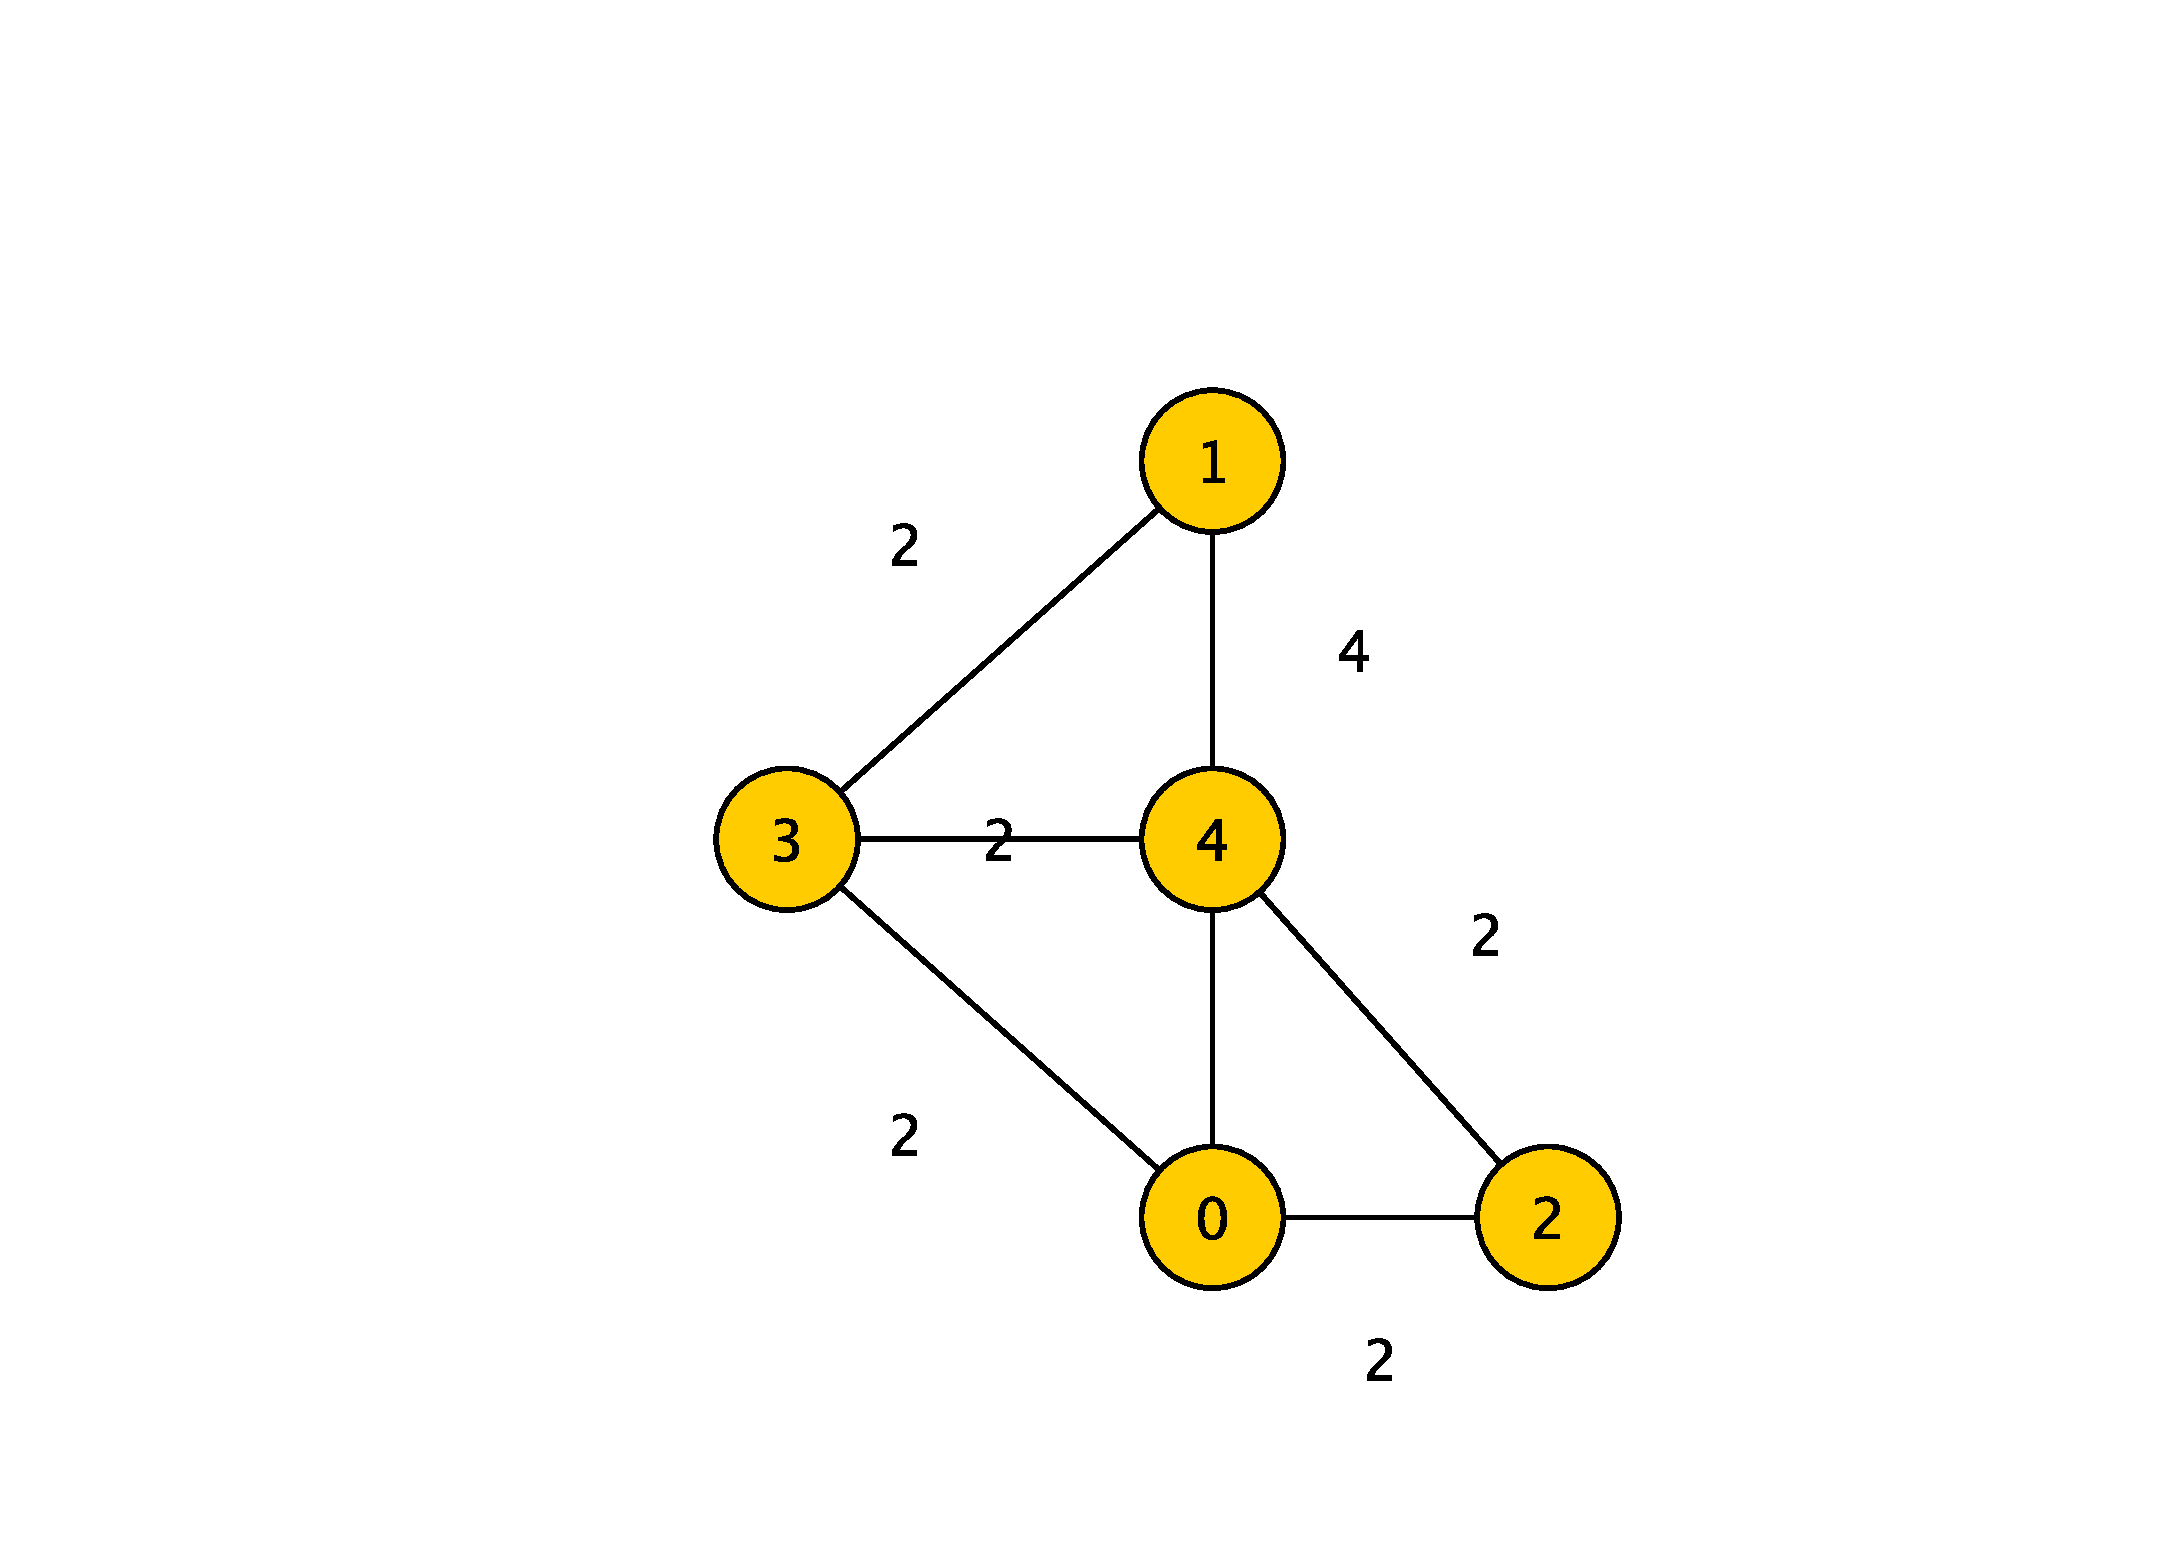
\includegraphics[scale=.15]{img/coarsening2.eps}
      \end{figure}
    \end{center}

    \column{.05\textwidth}{} 
    \begin{center}
      $\longrightarrow$  
    \end{center}    
    
    \column{.45\textwidth}{} 
    \begin{center}
      \begin{figure}[htbp]
        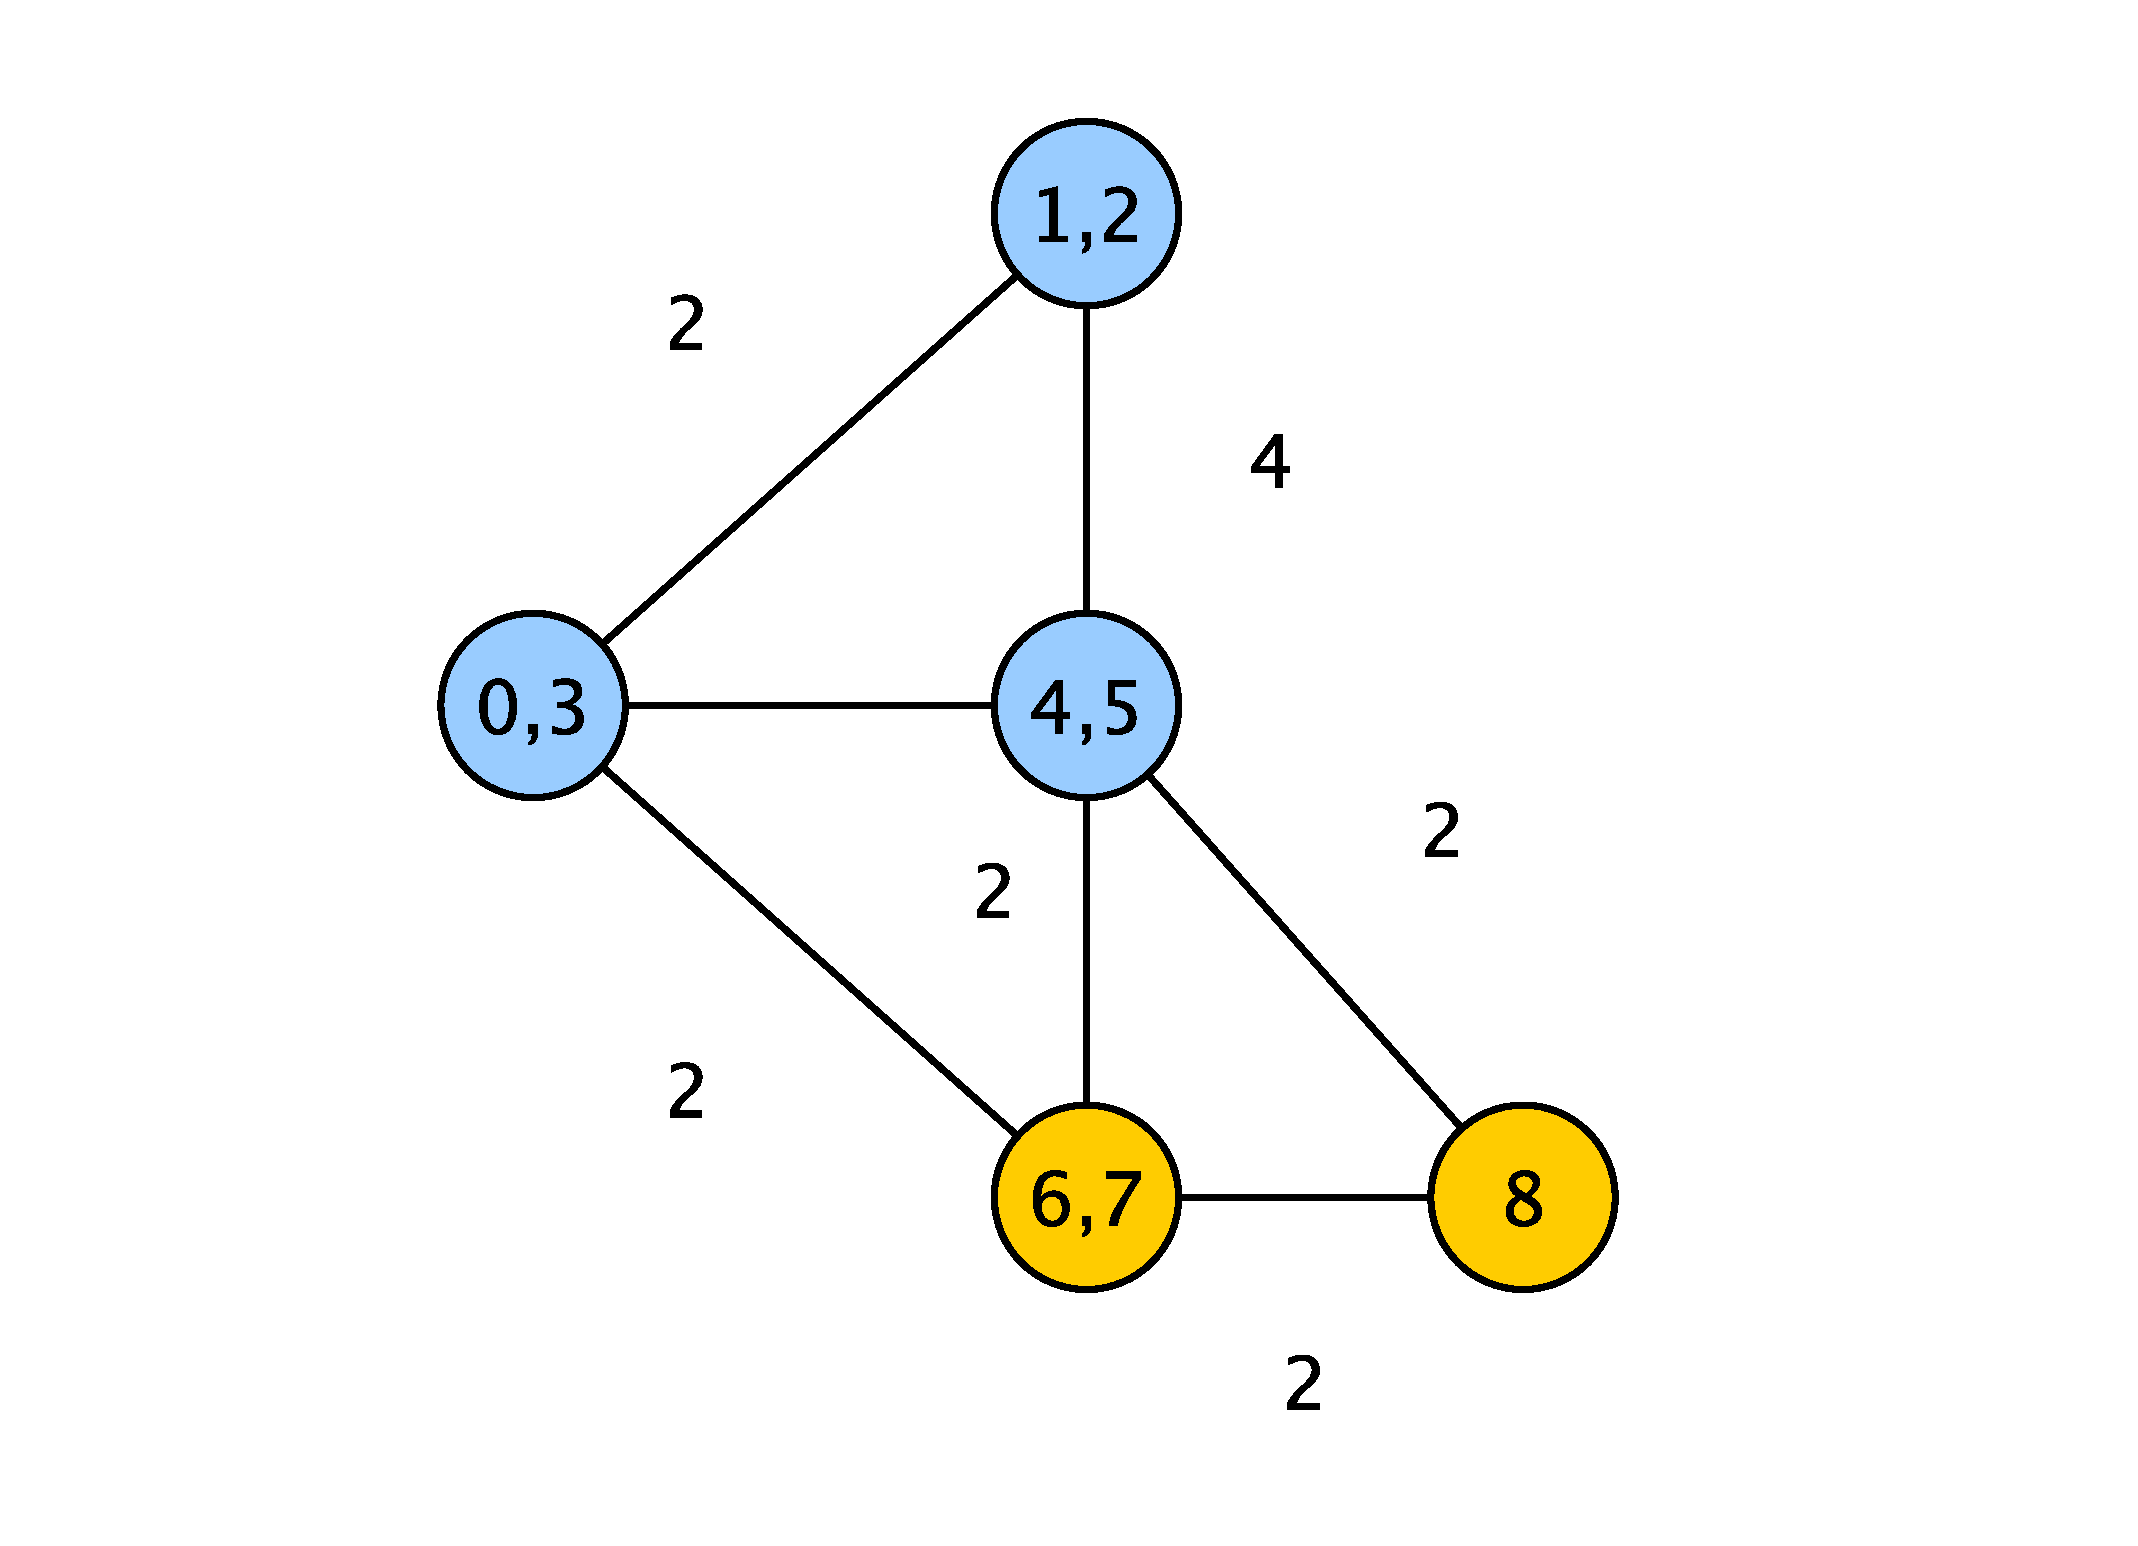
\includegraphics[scale=.15]{img/partition.eps}
      \end{figure}
    \end{center}

  \end{columns}
\end{frame}

\begin{frame}{Refinement}
  
  \begin{columns}[c]
    \column{.45\textwidth}{}
    \scriptsize
    \begin{center}
      \begin{figure}[htbp]
        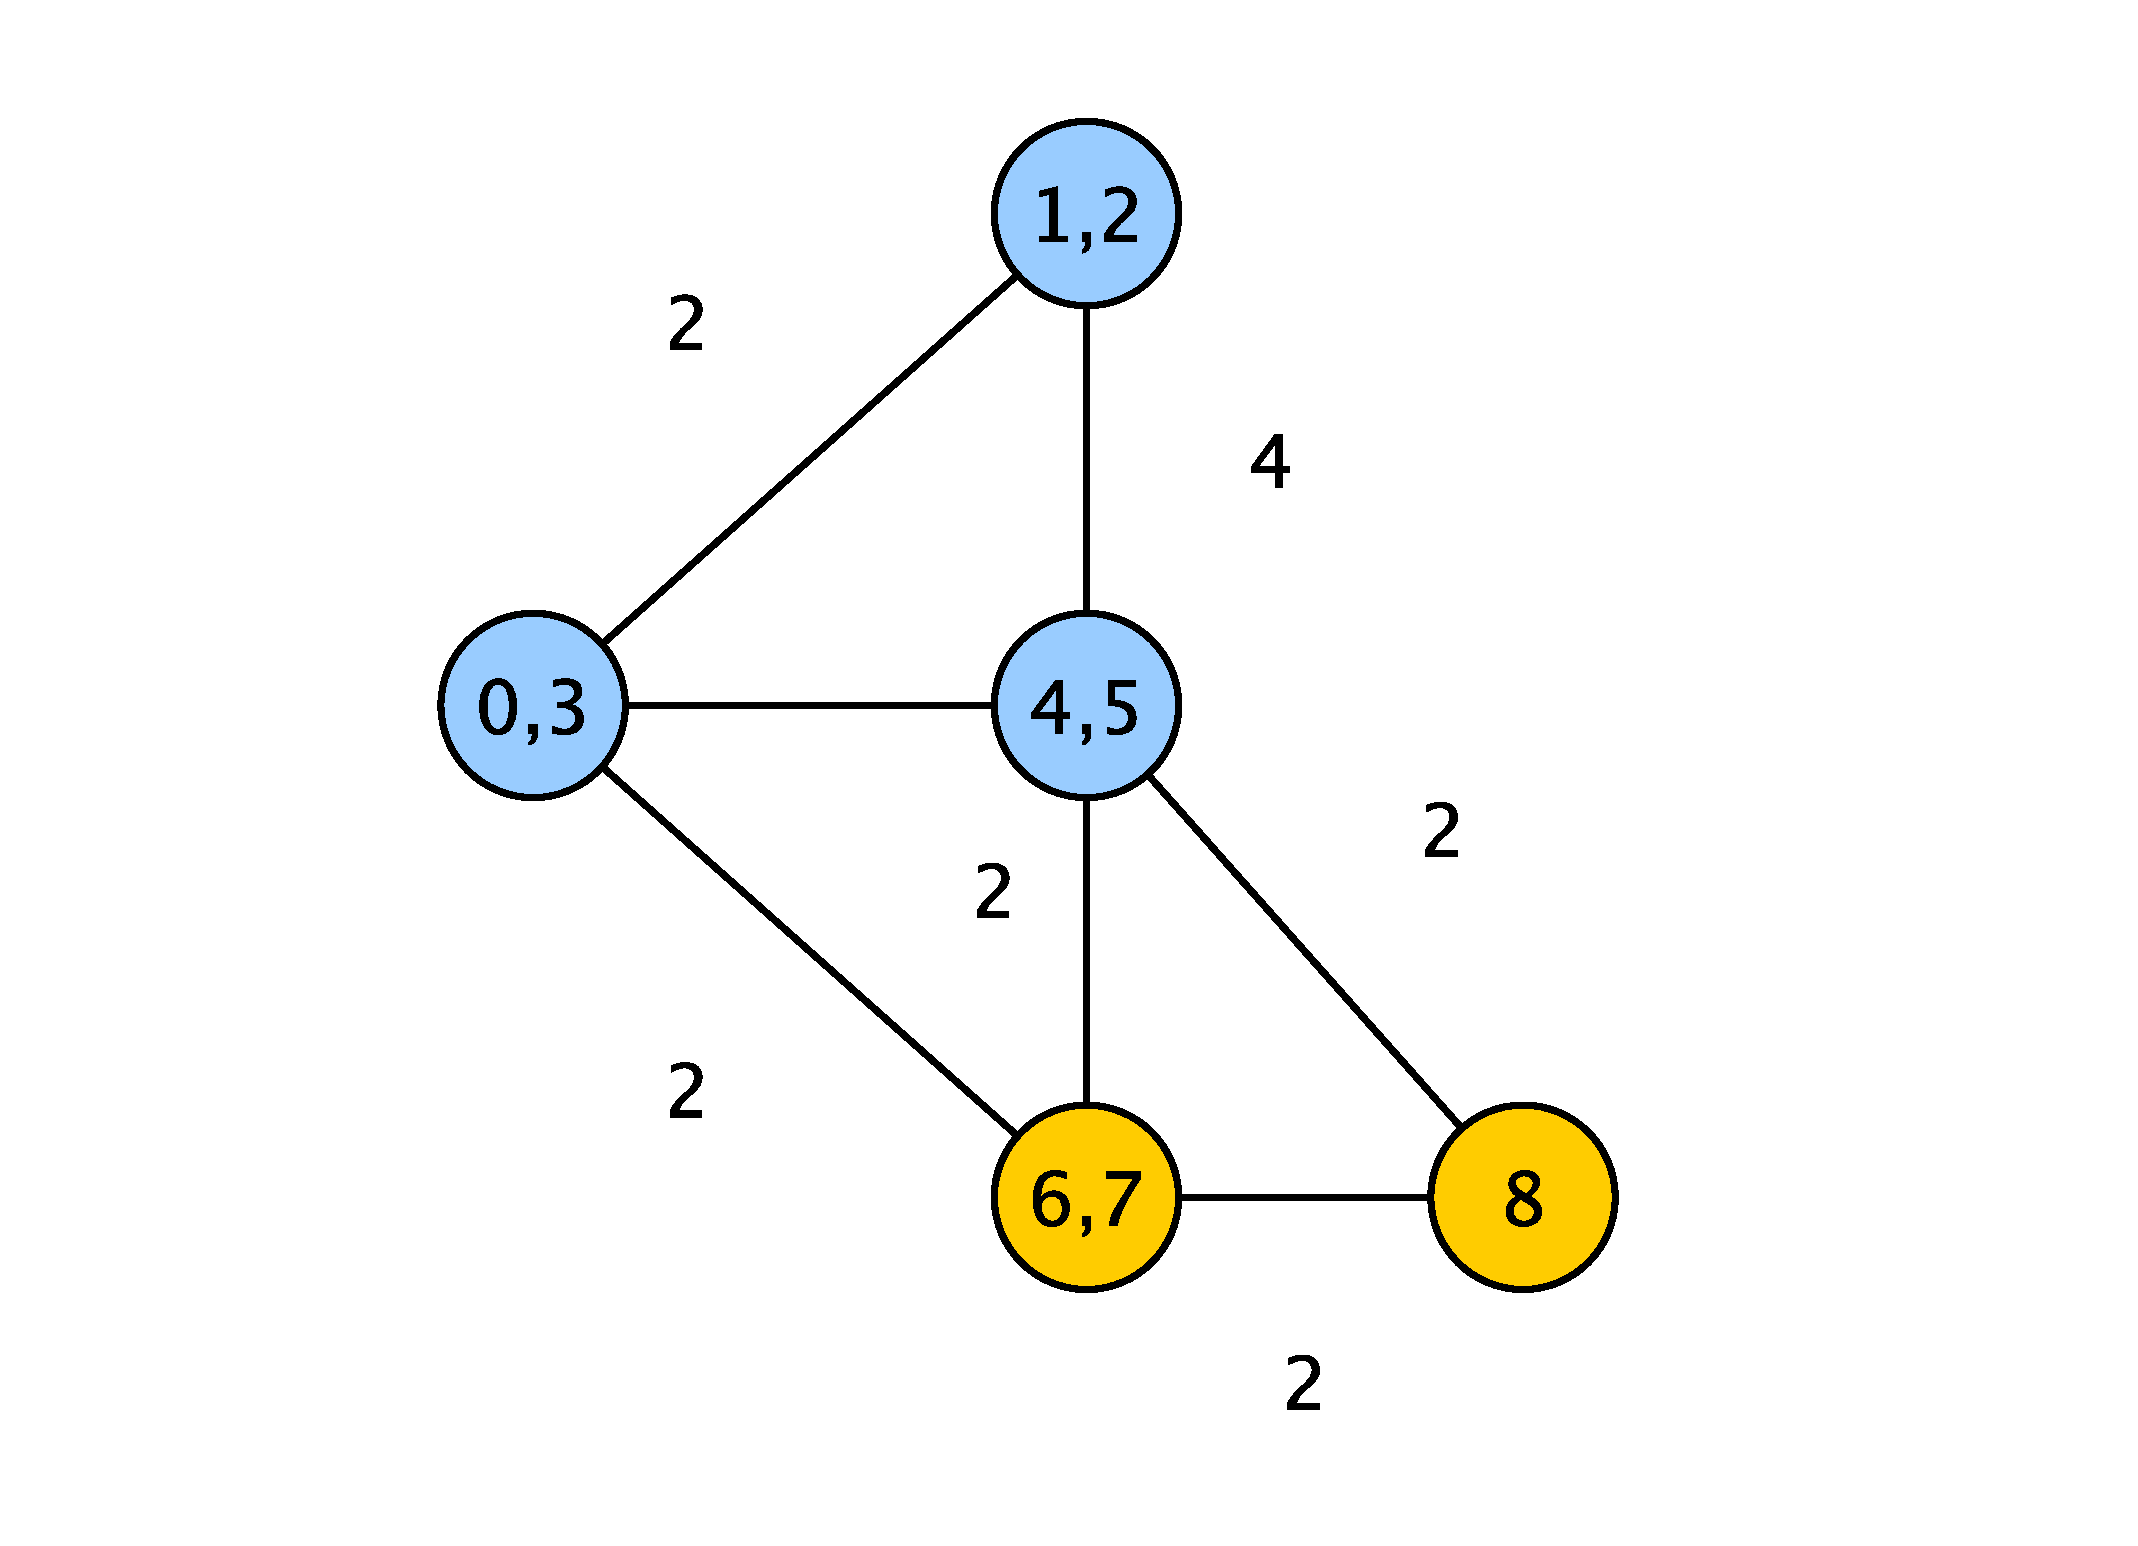
\includegraphics[scale=.15]{img/partition.eps}
      \end{figure}
    \end{center}

    \column{.05\textwidth}{} 
    \begin{center}
      $\longrightarrow$  
    \end{center}    
    
    \column{.45\textwidth}{} 
    \begin{center}
      \begin{figure}[htbp]
        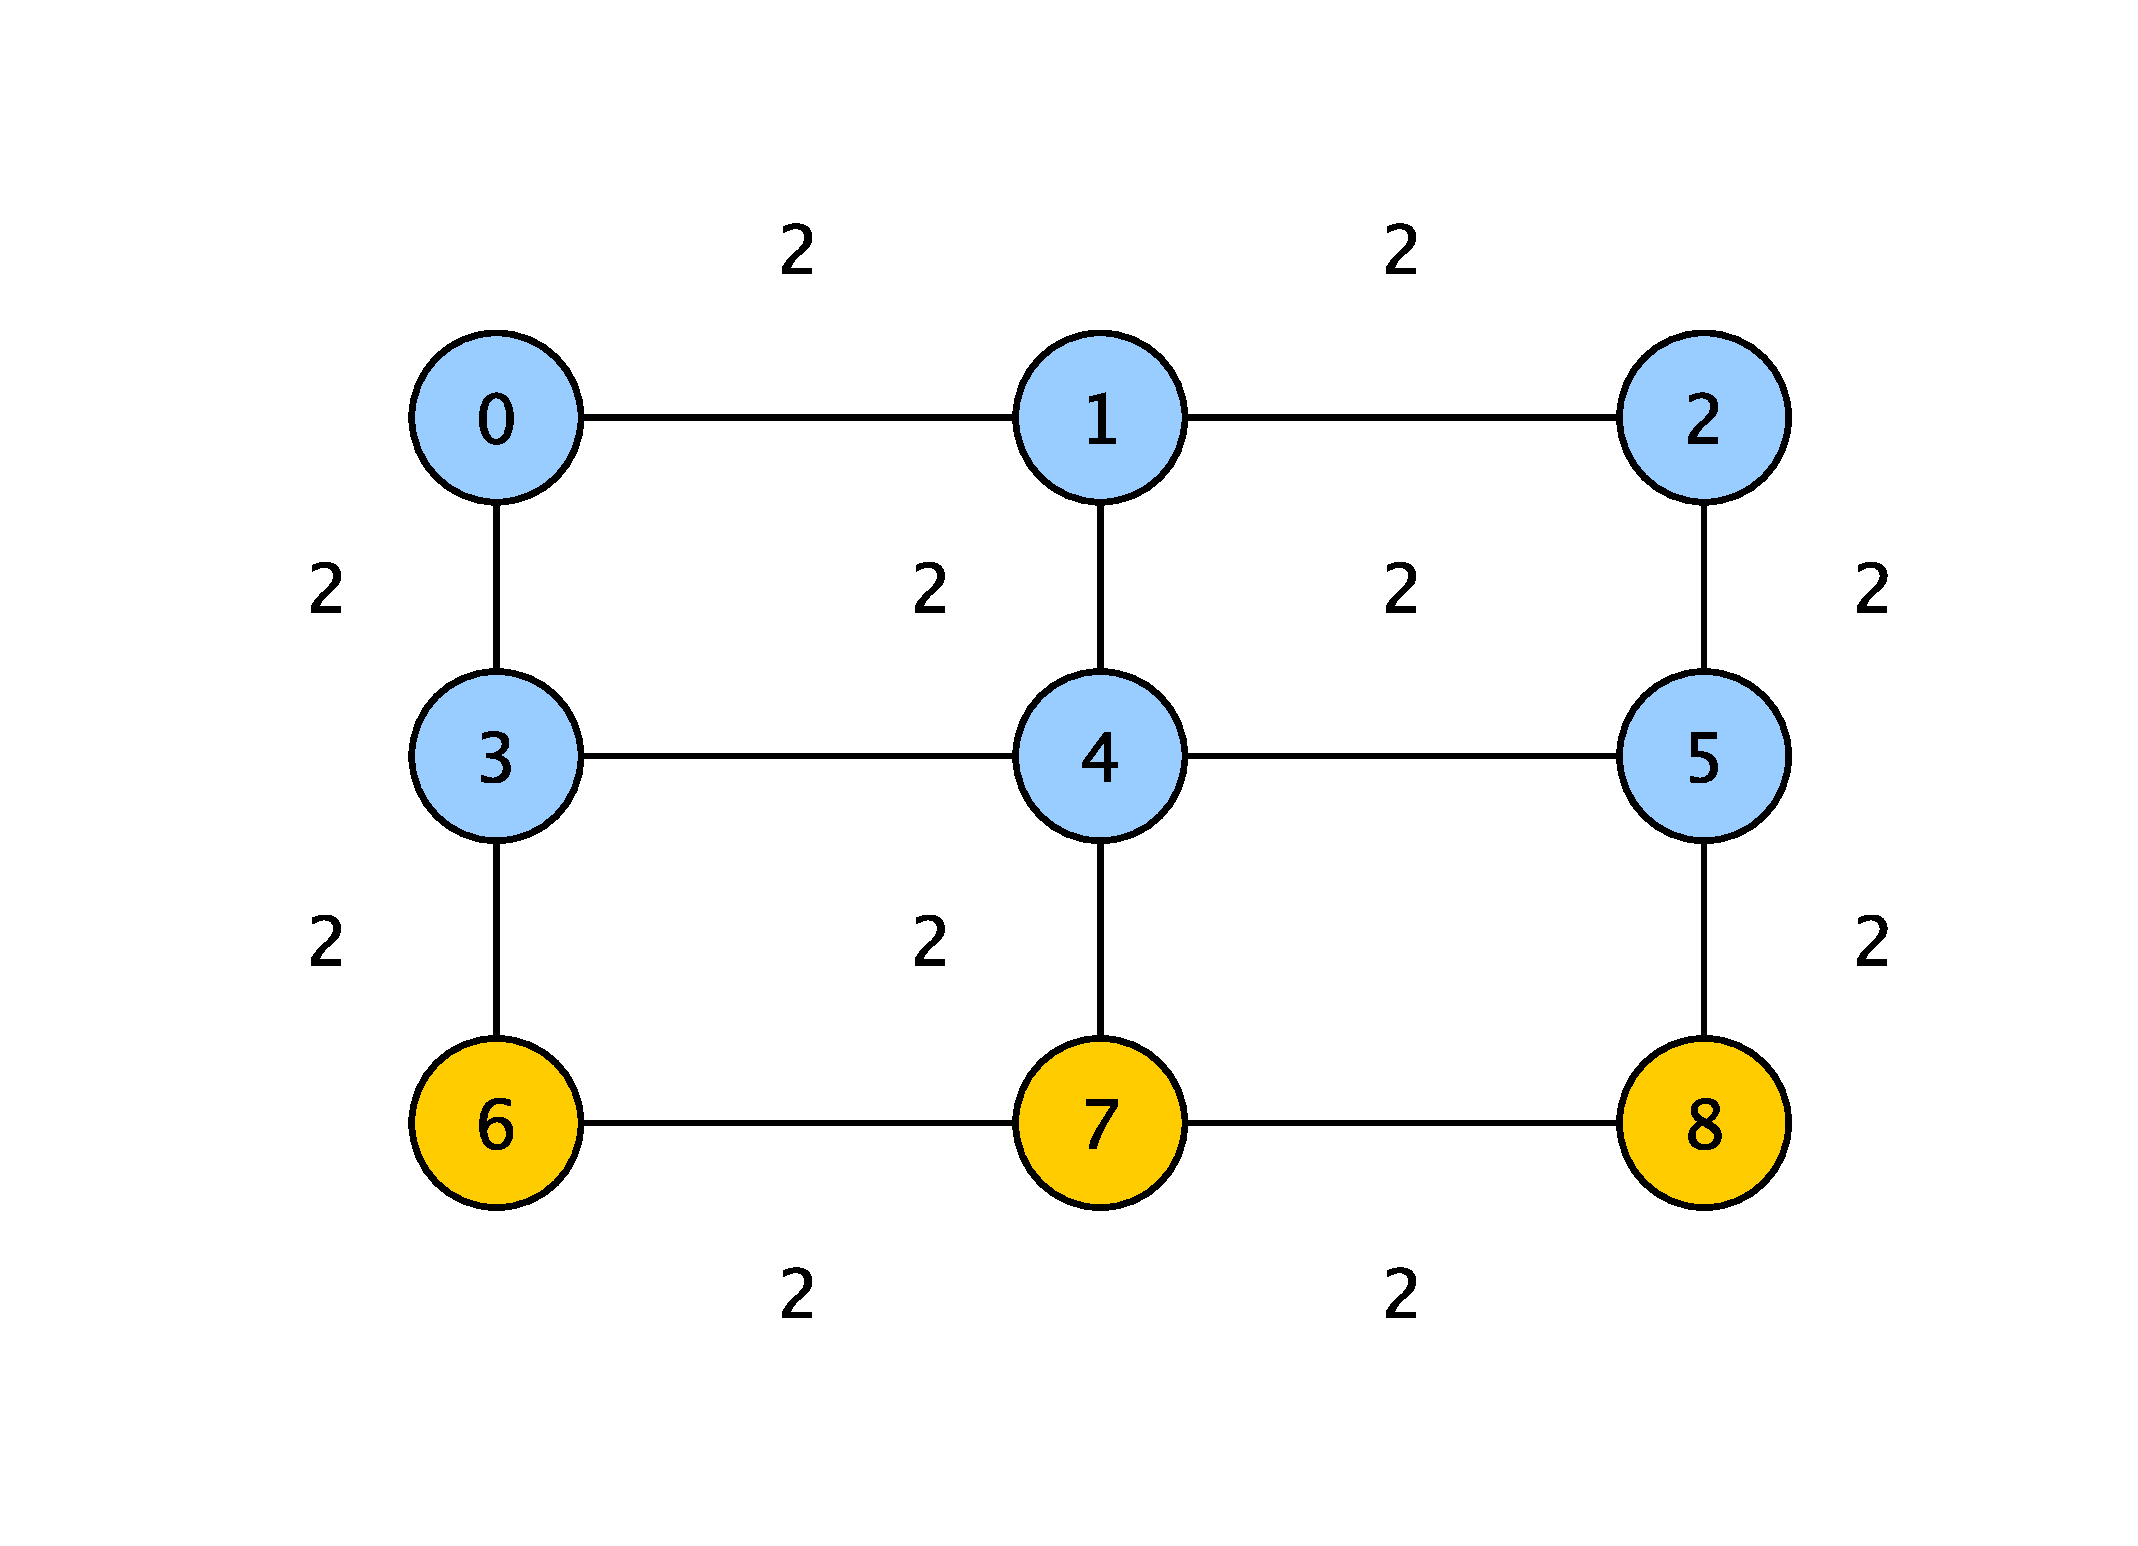
\includegraphics[scale=.15]{img/refinement.eps}
      \end{figure}
    \end{center}

  \end{columns}

\end{frame}



%-----------------------------------------------------------------------------
% System characteristics
%-----------------------------------------------------------------------------

\section{System characteristics}

\begin{frame}{Stampede Host}
\begin{table}[H]
\centering
\footnotesize
\begin{tabular}{| c | c |}\hline
Manufacturer & Intel\\ \hline
Model & Xeon E5-2680\\ \hline
$\mu$Arch & Sandy Bridge\\ \hline
Clock freq & 2.70 GHz\\ \hline
\#CPUs (sockets) & 2 \\ \hline
\#Cores/CPU & 8\\ \hline
\#Thread/Core & 1\\ \hline
L1 cache size/core & 32 KB\\ \hline
L2 cache size/core & 256 KB\\ \hline
L3 shared cache size/CPU & 20 MB\\ \hline
Main Memory/CPU & 16 GB\\ \hline
Vector width & 256 bits (AVX)\\ \hline
\end{tabular}
\caption{Intel Xeon E5-2680}
\end{table}
\end{frame}


\begin{frame}{Stampede Co-processor - Xeon Phi}
\begin{table}[H]
\centering
\footnotesize
\begin{tabular}{| c | c |}\hline
Manufacturer & Intel\\ \hline
Model & Xeon Phi SE10P\\ \hline
$\mu$Arch & Many Integrated Cores - MIC\\ \hline
Clock freq & 1.1 GHz\\ \hline
\#CPUs (sockets) & 1 \\ \hline
\#Cores/CPU & 61\\ \hline
\#Thread/Core & 4\\ \hline
L1 cache size/core & 32KB\\ \hline
L2 cache size/core & 512 KB\\ \hline
Main Memory/CPU & 8 GB\\ \hline
Vector width & 512 bits\\ \hline
\end{tabular}
\caption{Intel Xeon Phi}
\end{table}
\end{frame}

\begin{frame}{Important characteristics}
  \begin{itemize}
    \item Four hardware threads per core
    \item In-order dual issue pipeline
    \item Pipeline does not issue instructions from the same hardware
      context for two consecutive clock cycles
    \item Maximum issue rate only attainable with at least 2 threads per
      core
  \end{itemize}
\end{frame}

\begin{frame}{Xeon Phi Coprocessor Core\footnote{http://software.intel.com/en-us/articles/intel-xeon-phi-coprocessor-codename-knights-corner}}
  \begin{center}
  \begin{figure}[htbp]
      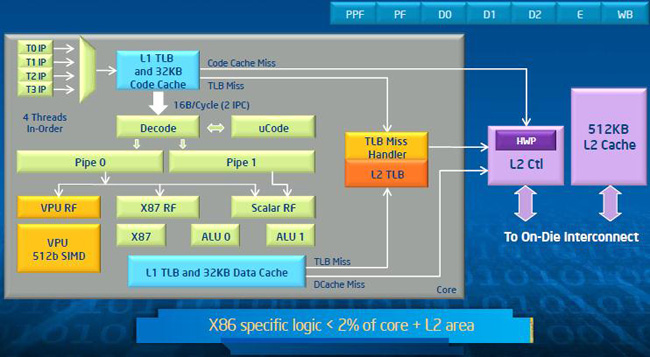
\includegraphics[scale=.45]{img/phi_arch.jpg}
  \end{figure}
  \end{center}
\end{frame}



%-----------------------------------------------------------------------------
% GMetis
%-----------------------------------------------------------------------------
\section{Results}

\begin{frame}{GMetis\footnote{USA-road-d.W.gr with 6262104 nodes and
  15248146 edges}}
\begin{center}
  \begin{figure}[htbp]
    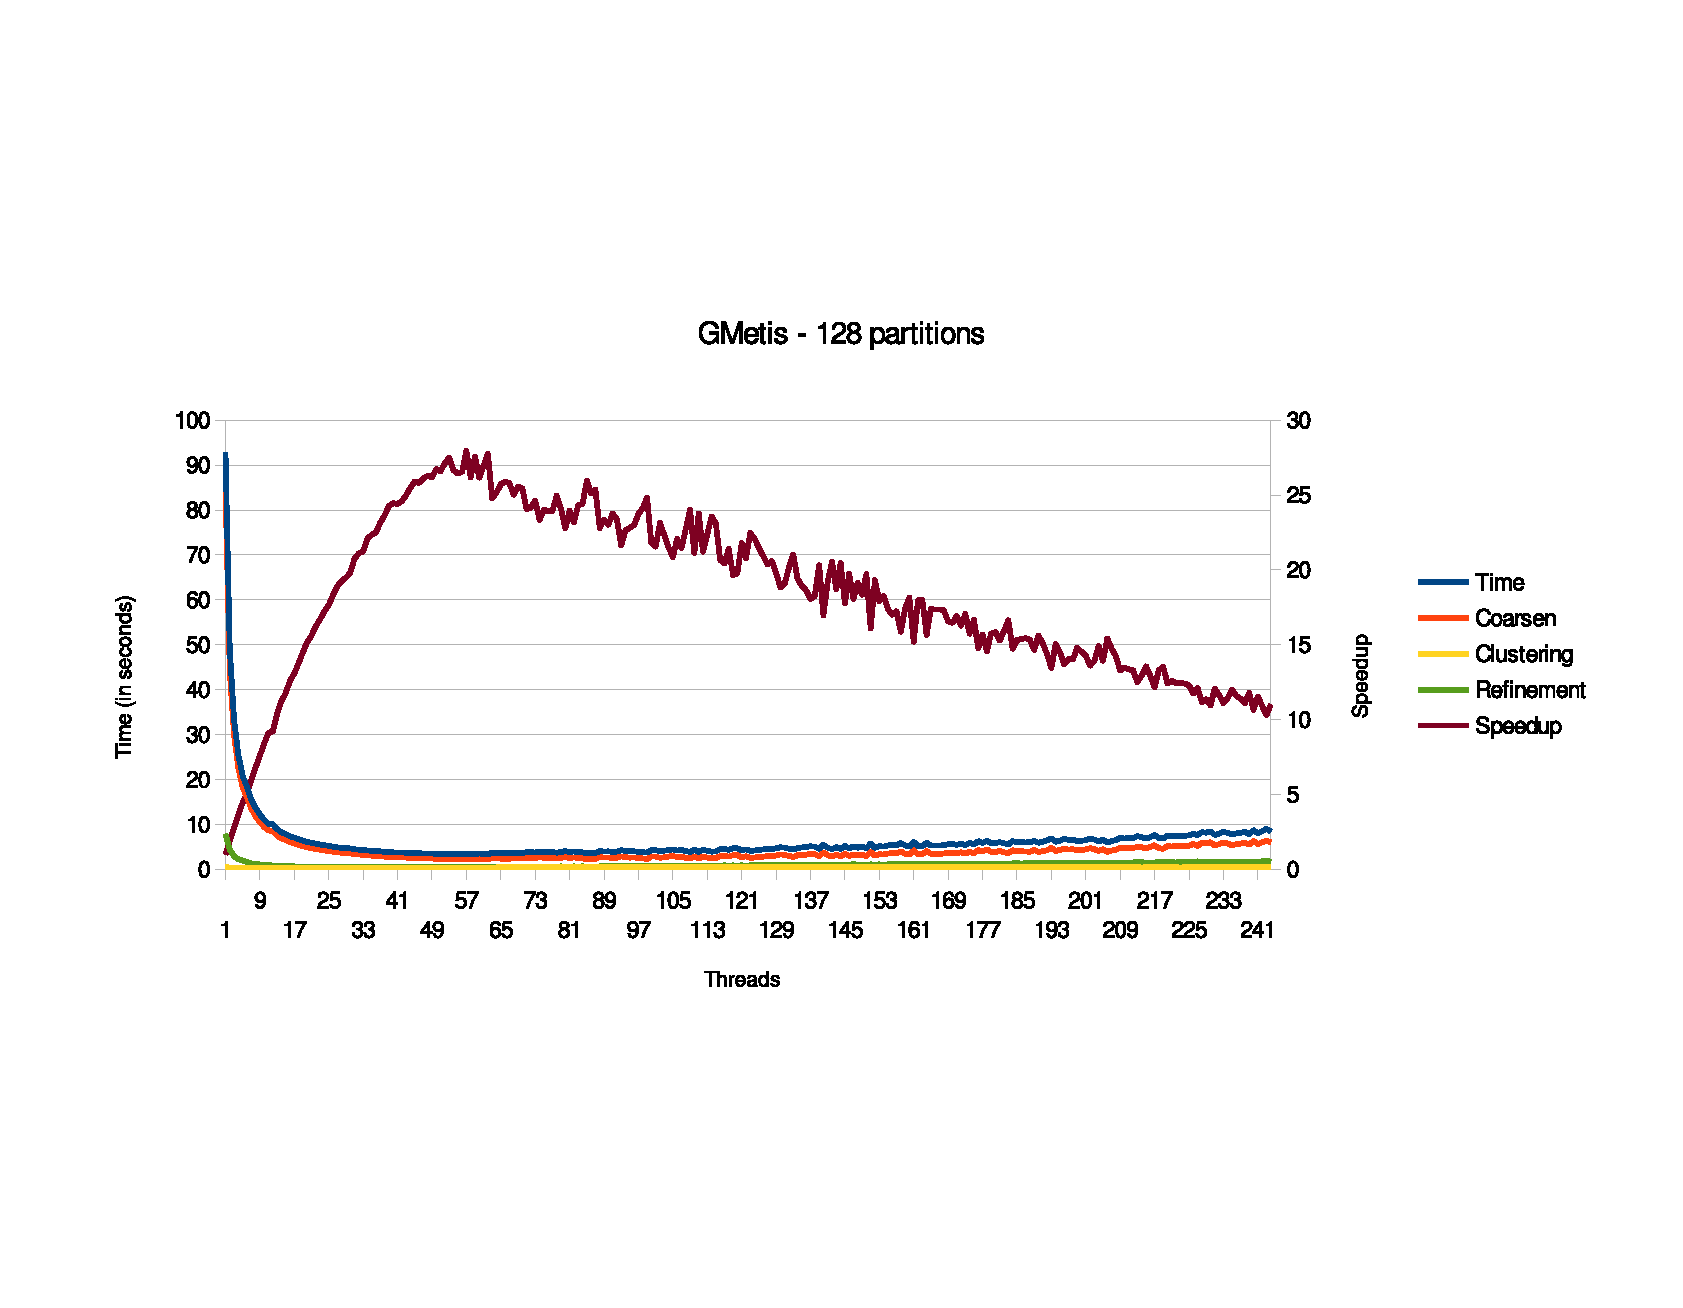
\includegraphics[scale=.45]{gmetis128.eps}
  \end{figure}
\end{center}
\end{frame}


%-----------------------------------------------------------------------------
% Mt-metis
%-----------------------------------------------------------------------------

\begin{frame}{Mt-metis}
\begin{center}
  \begin{figure}[htbp]
    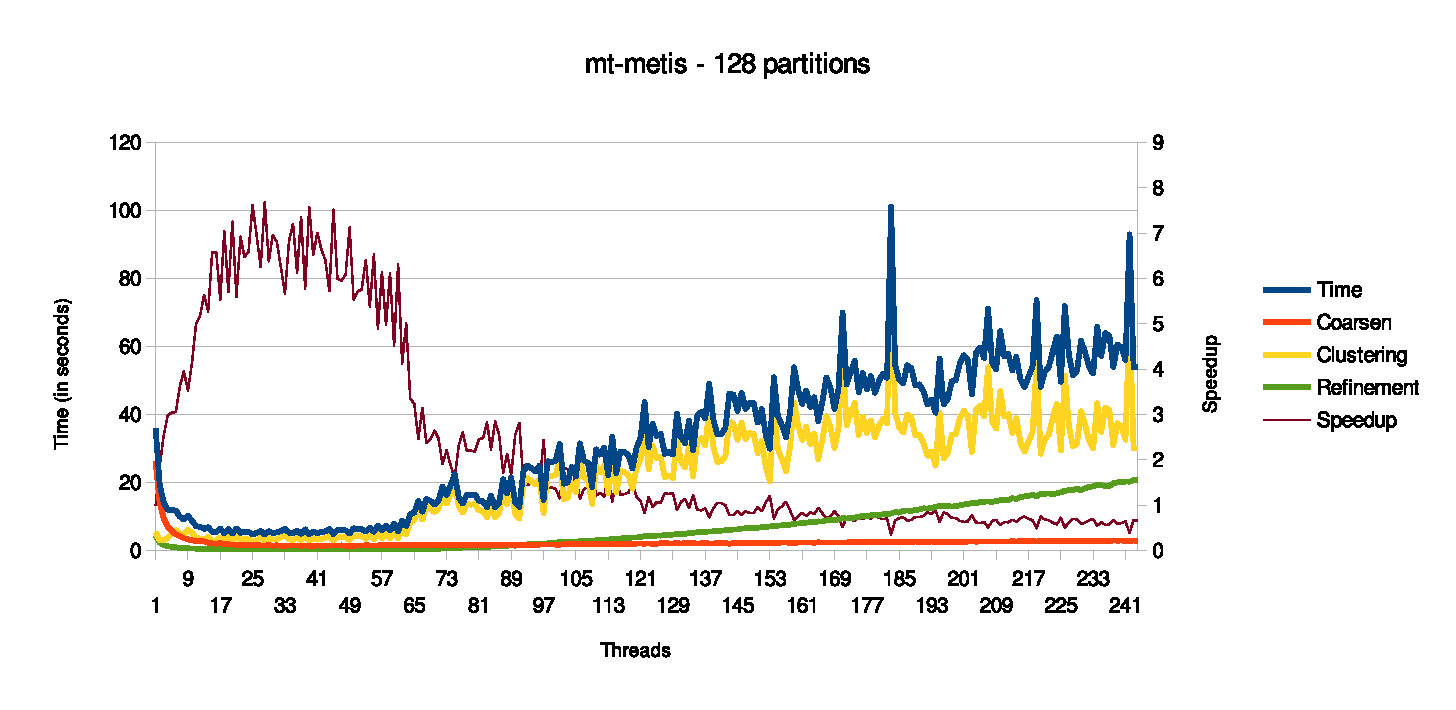
\includegraphics[scale=.45]{img/mtmetis128.eps}
  \end{figure}
\end{center}
\end{frame}


%-----------------------------------------------------------------------------
% Comparisons
%-----------------------------------------------------------------------------
\begin{frame}{Enhancements}
  \begin{itemize}
    \item Package Mapping (HW Topology)
    \begin{itemize}
      \item Default Mapping
      \item Load Balance
      \item Dense Package
    \end{itemize}
    \item Use of Random Match and Heavy Weight Match
    \item WorkList schedulers
    \item Software prefetching
\end{itemize}
\end{frame}

\begin{frame}{Metis Comparison}
\begin{center}
  \begin{figure}[htbp]
    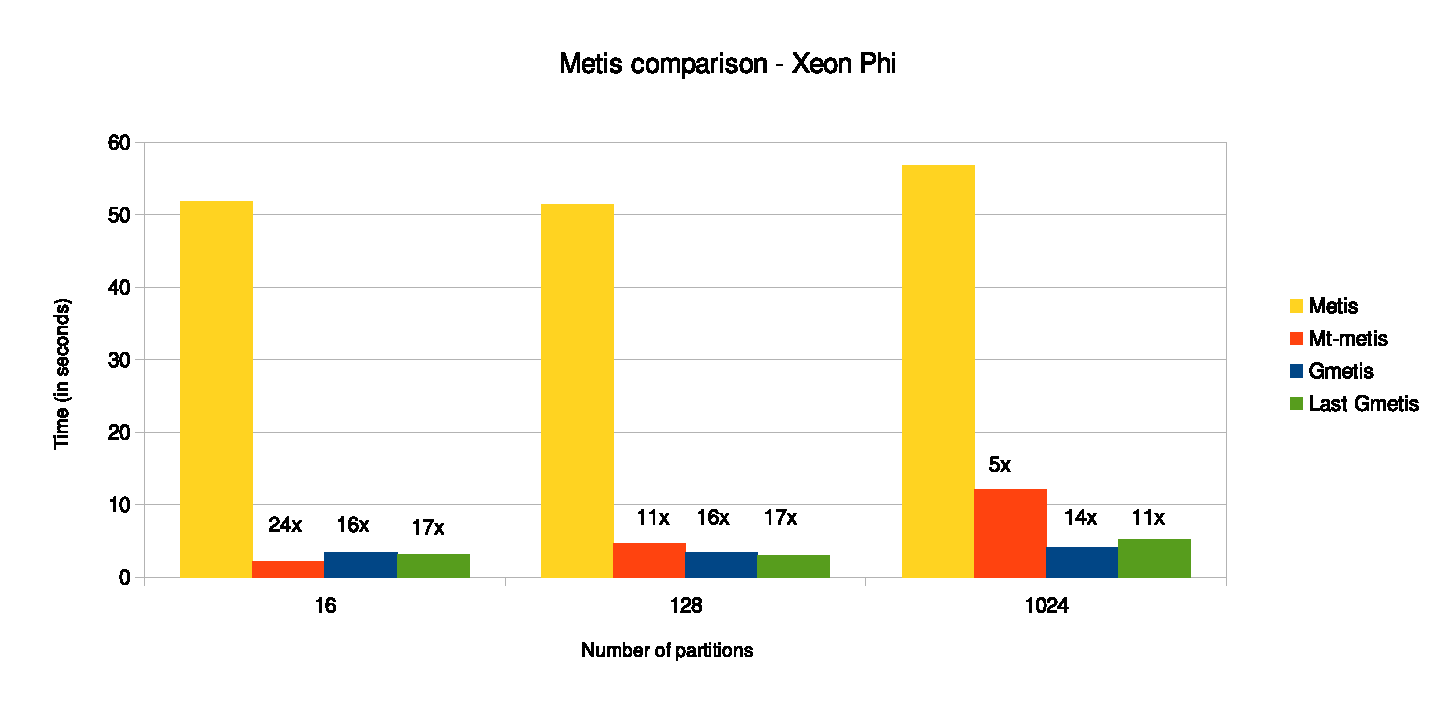
\includegraphics[scale=.45]{img/comparison.eps}
  \end{figure}
\end{center}
\end{frame}

\begin{frame}{Edgecut comparison}
\begin{center}
  \begin{figure}[htbp]
    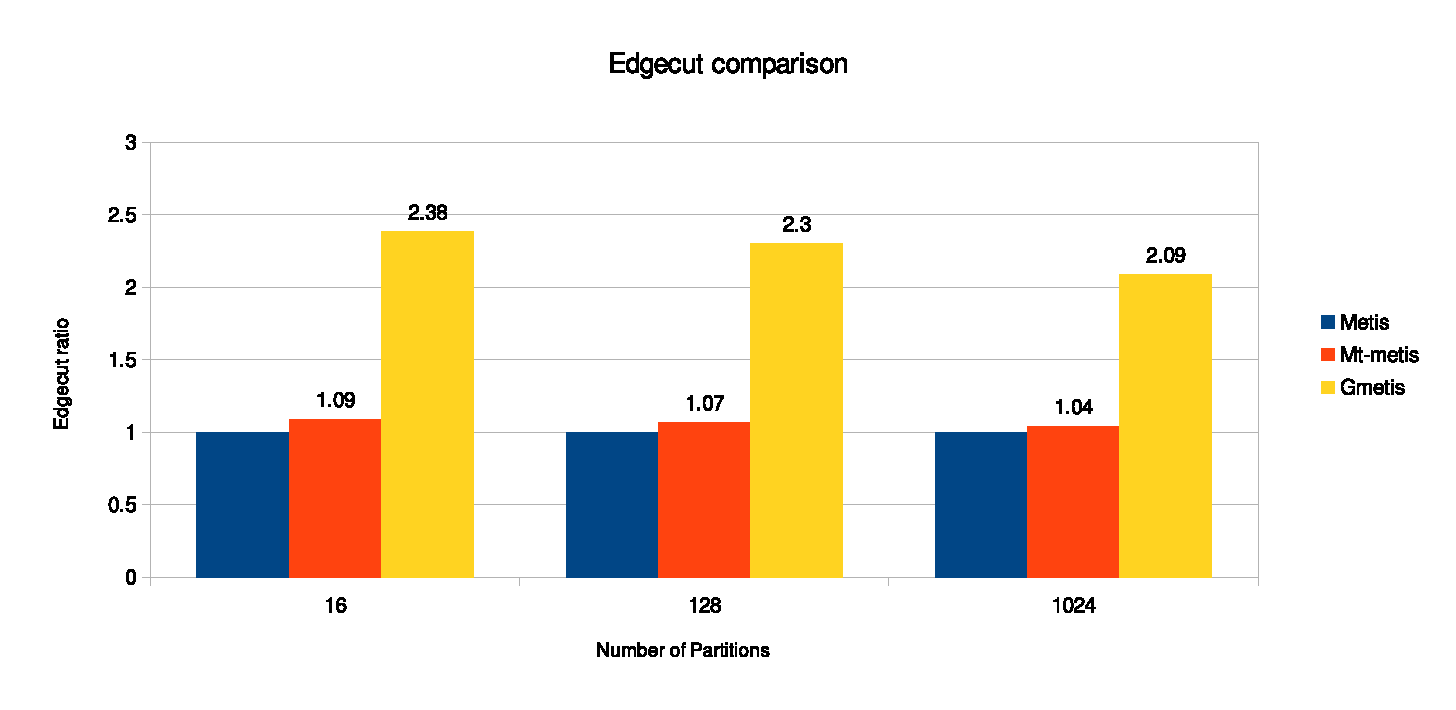
\includegraphics[scale=.45]{img/edgecut.eps}
  \end{figure}
\end{center}
\end{frame}



%-----------------------------------------------------------------------------
% Conclusion
%-----------------------------------------------------------------------------

\section{Conclusion}

\begin{frame}{Conclusion}
\begin{itemize}
  \item Metis and mt-metis have better edgecut;
  \item Metis and mt-metis have lower runtimes for a smaller number of partitions;
  \item GMetis is faster for a high number of partitions;
  \item Metis graph partitioning algorithm is not suitable to run on MIC as it does not use SIMD extensions;
  % no entanto, não é razão para problemas de escalabilidade
  \item Lack of software/profilers made progress difficult;
\end{itemize}
\end{frame}

% 2 ou 3 dias downtime - maintenance do stampede
% hpctoolkit - lixo
% perfexpert - depende do hpctoolkit
% vtune nao é suportado
% PAPI e timers à pata
% Minor version do ICC e troca de compiladores


%-----------------------------------------------------------------------------
% End Page 
%-----------------------------------------------------------------------------

\begin{frame}
  \titlepage
  \begin{center}
  \huge ?
  \end{center}
\end{frame}

\end{document}
